%!TEX root = ../dynamics.tex
\section{Analyzing the Features Affecting Batch Throughput}
\label{sec:throughput}
Next we turn our attention to analyzing the factors that influence the fast progress (or completion) of a batch, how they change, interplay, and their scope overtime.
\subsection{A Machine Learning Approach}
In order to conduct this analysis, we define the task of batch throughput prediction as a regression problem.  Some of the  29  features we use for this task were used in the previous section to classify HIT type.  We describe the remaining ones in appendix A. The value  we want to predict (i.e.,   $DIFF\_HIT$) is the batch \emph{throughput}, that is, numbers of HITs that  a given batch would have completed within the next time frame of 1 hour.

In detail, to predict the throughput of a batch at time $T$, we train a Random Forest Regression model with samples taken in the range $[T-\delta, T)$ where $\delta$ is a time window that we are   considering directly prior to time $T$. The rational behind this approach is that the throughput is directly linked to current and previous market situation. 
The remaining question is: ``how much historical data we can consider whiteout adding too much noise?" and for that we proceed by varying $\delta$.
In this process we compute the coefficient of determination  $R^2$ score \cite{sklearnweb, sklearn}.
In this experiment we considered  data from June-October 2014 and hourly observations (see Section \ref{sec:tracker}), from which we uniformly sampled 50 time points for evaluation purposes. Finally, for each time point we considered a training time frame $\delta$ ranging from 1 hour to 24 hours. 

In Figure \ref{fig:accuracy} we see how the computed evaluation score reaches its highest values when using the latest 4 hours as a training time frame, then decreases when we increase the time frame, to finally again increase and stabilize when we use up to 24 hours training evidence.
Note that the score is relatively low especially for batches with low throughput HITs. The prediction works best for larger batches having a large momentum as Figure \ref{fig:pred} suggests.

\begin{figure}[tb]
	\centering
		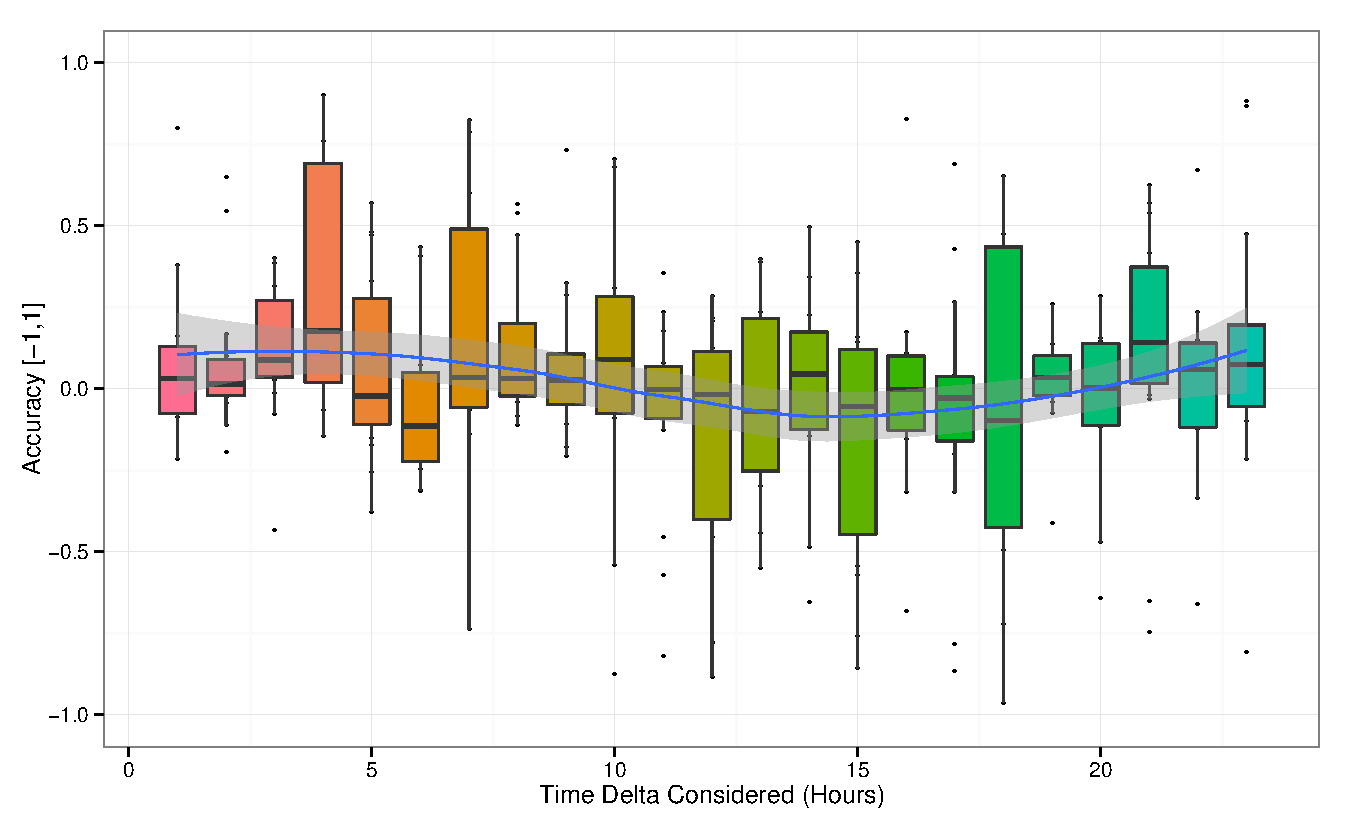
\includegraphics[width=0.48\textwidth]{figures/ML_accuracy}
	\caption{Score ($R^2$) of the throughput prediction when considering larger time spans as training sets. The red dots are average values, while the boxes represents the median, first and third quartiles.}
	\label{fig:accuracy}
\end{figure}

\begin{figure}[tb]
	\centering
		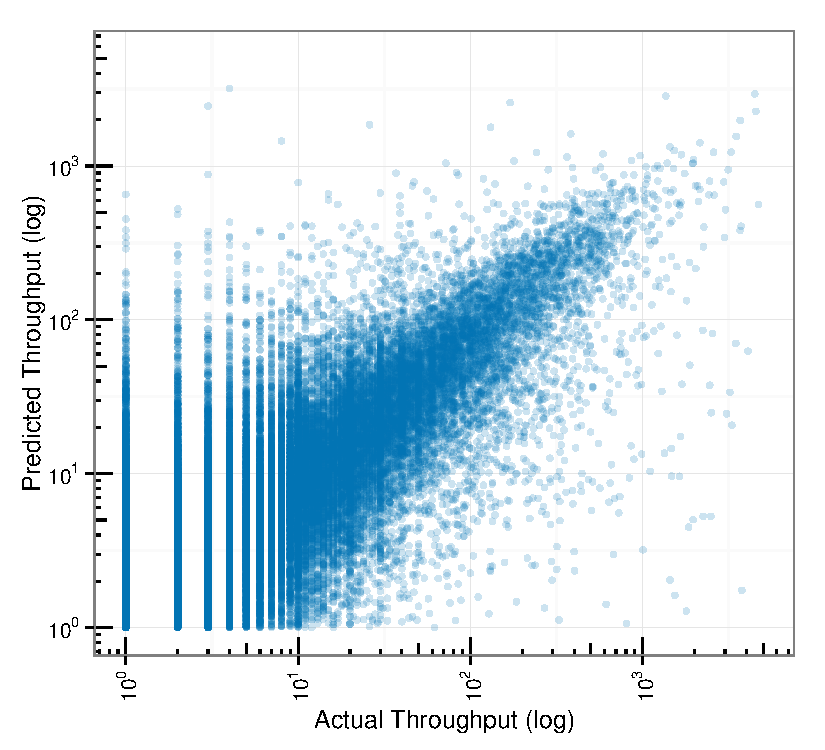
\includegraphics[width=0.48\textwidth]{figures/predictions_3}
	\caption{Prediction vs actual throughput values. Prediction is more accurate for larger throughput values. This suggests that the throughput will remain high until the batch gets smaller.}
	\label{fig:pred}
\end{figure}

\begin{figure}[tb]
	\centering
		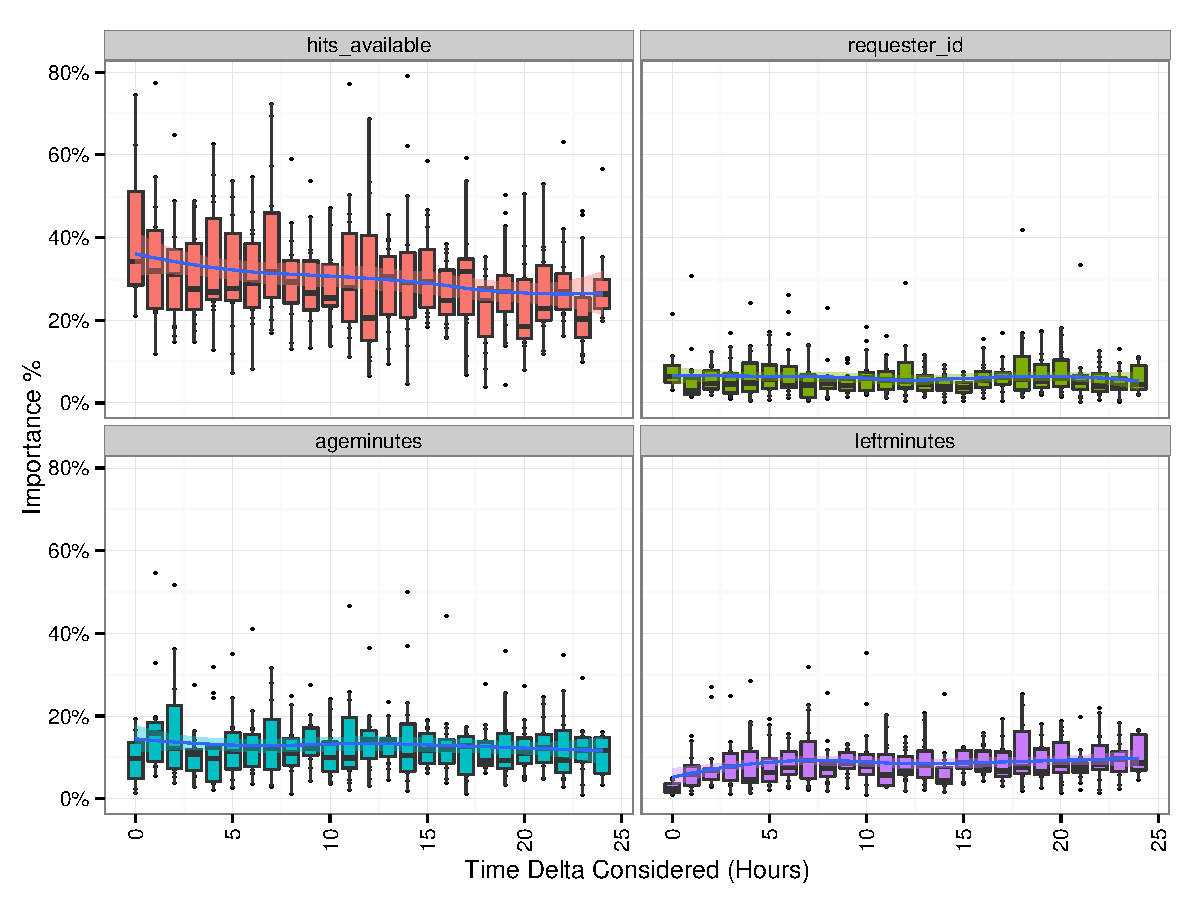
\includegraphics[width=0.5\textwidth]{figures/importances}
	\caption{Computed feature importance when considering larger training sets for the prediction.}
	\label{fig:importances}
\end{figure}


In order to understand  changes in throughput prediction we  look at  feature importance that we computed during   the training phase. Figure \ref{fig:importances} shows the  contribution of each feature and how it varied along when we increased the training time frame.
The most important feature is $HIT\_Available$, that is, the current size of the batch. Indeed, as observed by previous work, larger batches tend to attract more workers\cite{mturk,crowddb}. This feature becomes less important when we consider longer periods, partly because of  noise, but, most importantly, because of other features like $Start\_time$ and $left\_minutes$ starting to encode additional facts and suggests that the crowd is sensitive to the newly posted HITs, or how \emph{fresh} the HITs are. To better understand this phenomena, in the next section we conduct an analysis on what attracts the workforce to the the platform.

